\section{NTLM authentication}

LM and  NTLM here are the hash names, and NTLMv1 and NTLMv2 are authentication  protocols that utilize the LM or NT hash. Below is a quick comparison  between these hashes and protocols, which shows us that, while not  perfect by any means, Kerberos is often the authentication protocol of  choice wherever possible. It is essential to understand the difference  between the hash types and the protocols that use them.

\begin{tabular}{|l|l|l|l|l|}
 \hline \hline
 Hash     & Crypto    & Mutual & Msg Type & Trusted  \\
 Protocol & technique &  Authn &          & 3d Party \\
 \hline \hline
 NTLM & Sym  & No & Rnd nbr & DC \\
 NTLMv1 & Sym  & No & MD4 hash, rnd nbr & DC \\
 NTLMv2 & Sym  & No & MD4 hash, rnd nbr & DC \\
 Kerberos & Sym \& Asym & Yes & Encrypted ticket using DES, MD5 & DC, KDC \\
 \hline \hline
\end{tabular}

\subsection{LM}

LAN Manager (LM) hashes are the oldest password storage  mechanism used by the
Windows operating system. LM debuted in 1987 on  the OS/2 operating system. If
in use, they are stored in the SAM  database on a Windows host and the
\gls{win:NTDS.DIT} database on a Domain  Controller. Due to significant security weaknesses in the hashing  algorithm used for LM hashes, it has been turned off by default since  Windows Vista/Server 2008. However, it is still common to encounter,  especially in large environments where older systems are still used.  Passwords using LM are limited to a maximum of 14  characters. Passwords are not case sensitive and are converted to  uppercase before generating the hashed value, limiting the keyspace to a  total of 69 characters making it relatively easy to crack these hashes  using a tool such as Hashcat.

Before hashing, a 14 character password is first split into two
seven-character chunks. If the password is less than fourteen  characters, it
will be padded with NULL characters to reach the correctvalue. Two DES keys
are created from each chunk. These chunks are then  encrypted using the string
\verb+KGS!@#$%+, creating two 8-byte  ciphertext values. These two values are
then concatenated together,  resulting in an LM hash. This hashing algorithm
means that an attacker  only needs to brute force seven characters twice
instead of the entire  fourteen characters, making it fast to crack LM hashes
on a system with  one or more GPUs. If a password is seven characters or less,
the second  half of the LM hash will always be the same value and could even be
determined visually without even needed tools such as Hashcat. The use  of LM
hashes can be disallowed using Group Policy. An LM hash takes the form of
\verb+299bd128c1101fd6+.

\subsection{NTHash (NTLM)}

NT LAN Manager (NTLM) hashes are used on modern Windows  systems. It is a
challenge-response authentication protocol and uses  three messages to
authenticate: a client first sends a \verb+NEGOTIATE_MESSAGE+ to the server,
whose response is a \verb+CHALLENGE_MESSAGE+ to verify the client's identity.
Lastly, the client responds with an \verb+AUTHENTICATE_MESSAGE+.  

\begin{figure}
  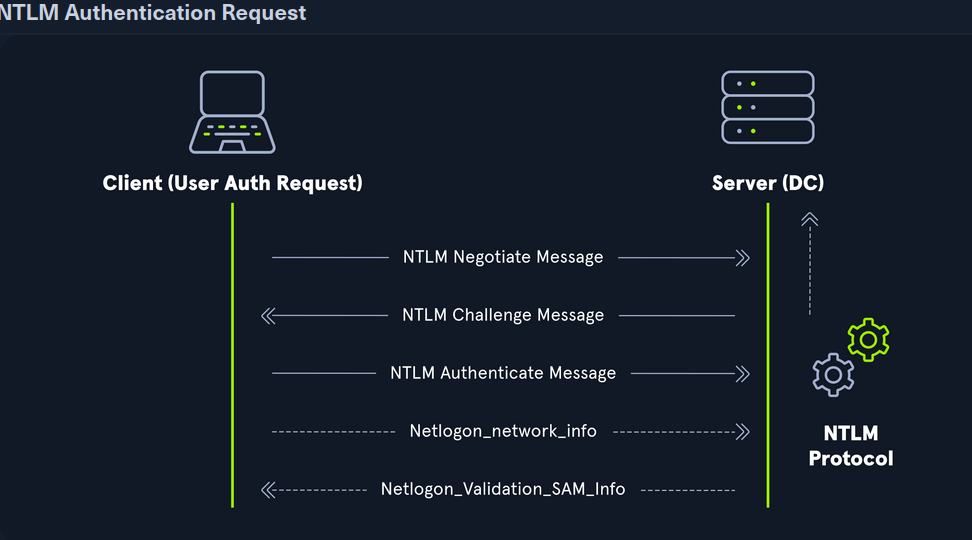
\includegraphics[width=\linewidth]{windows_knowledge/authentication/images/ntlm.png}
  \caption{NTLM protocol}
  \label{fig:ntlm-protocol}
\end{figure}


These hashes are stored locally in the SAM database or the \gls{win:NTDS.DIT}
database file on a Domain Controller. The protocol has two hashed  password
values to choose from to perform authentication: the LM hash (as discussed
above) and the NT hash, which is the MD4 hash of the little-endian UTF-16 value
of the password. The algorithm can be  visualized as:
$$(UTF-16-LE(password))$$.


Even though they are considerably stronger than LM hashes (supporting the entire Unicode character set of 65,536 characters), they can still  be brute-forced offline relatively quickly using a tool such as Hashcat. NTLM is also vulnerable to the  pass-the-hash attack, which means an attacker can use just the NTLM hash to authenticate to  target systems where the user is a local admin without needing to know  the cleartext value of the password.

An NT hash takes the form of \verb+b4b9b02e6f09a9bd760f388b67351e2b+, which is the second half of the full NTLM hash. 

An NTLM hash looks like
this:

\begin{verbatim}
Rachel:500:aad3c435b514a4eeaad3b935b51304fe:e46b9e548fa0d122de7f59fb6d48eaa2:::
\end{verbatim}

Looking at the hash above, we can break the NTLM hash down into its individual parts:
\begin{itemize}
    \item  \verb+Rachel+ is the username
    \item  \verb+500+ is the Relative Identifier (RID). 500 is the known RID for the administrator account
    \item  \verb+aad3c435b514a4eeaad3b935b51304fe+ is the LM hash and, if LM hashes are disabled on the system, can not be used for anything
    \item  \verb+e46b9e548fa0d122de7f59fb6d48eaa2+ is the NT hash. This hash can either be cracked offline or used for a pass-the-hash attack.
\end{itemize}

\subsection{NTLMv1 (Net-NTMLv1)}

The NTLM protocol performs a challenge/response between a server and  client using the NT hash. 

NTLMv1 uses both the NT and the LM hash, which can make it easier to "crack" offline after capturing a hash using a tool such as Responder or via an NTLM relay attack  

The protocol is used for network authentication, and the Net-NTLMv1 hash itself is created from a challenge/response algorithm. The server sends the client an 8-byte  random number (challenge), and the client returns a 24-byte response.  These hashes can NOT be used for pass-the-hash attacks. The algorithm  looks as follows:

\begin{verbatim}
C = 8-byte server challenge, random
K1 | K2 | K3 = LM/NT-hash | 5-bytes-0
response = DES(K1,C) | DES(K2,C) | DES(K3,C)
\end{verbatim}


\subsection{NTLMv2 (Net-NTLMv2)}

NTLMv2 sends two responses to the 8-byte challenge received by the server.
These responses contain a 16-byte \verb+HMAC-MD5+ hash of the challenge, a
randomly generated challenge from the client, and an \verb+HMAC-MD5+ hash of the user's credentials. 

A  second response is sent, using a variable-length client challenge including the current time, an 8-byte random value, and the domain name.  

The algorithm is as follows:

\begin{verbatim}
SC = 8-byte server challenge, random
CC = 8-byte client challenge, random
CC* = (X, time, CC2, domain name)
v2-Hash = HMAC-MD5(NT-Hash, user name, domain name)
LMv2 = HMAC-MD5(v2-Hash, SC, CC)
NTv2 = HMAC-MD5(v2-Hash, SC, CC*)
response = LMv2 | CC | NTv2 | CC*
\end{verbatim}


We can see that developers improved upon v1 by making NTLMv2 harder to crack and giving it a more robust algorithm made up of multiple stages. 


\subsection{Domain Cached Credentials (MSCache2)}
In an AD environment, the authentication methods mentioned in this  section and
the previous require the host we are trying to access to  communicate with the
"brains" of the network, the Domain Controller.  Microsoft developed the MS
Cache v1 and v2 algorithm (also known as Domain Cached Credentials  (DCC) to
solve the potential issue of a domain-joined host being unable  to communicate
with a domain controller (i.e., due to a network outage  or other technical
issue) and, hence, NTLM/Kerberos authentication not  working to access the host
in question. Hosts save the last ten hashes for any domain users that
successfully log into the machine in the
\verb+HKEY_LOCAL_MACHINE\SECURITY\Cache+  registry key. These hashes cannot be used in pass-the-hash attacks.  Furthermore, the hash is very slow to crack with a tool such as Hashcat,  even when using an extremely powerful GPU cracking rig, so attempts to  crack these hashes typically need to be extremely targeted or rely on a  very weak password in use. 

These hashes can be obtained by an attacker or pentester after gaining local
admin access to a host and have thefollowing format:
\begin{verbatim}
$DCC2$10240#bjones#e4e938d12fe5974dc42a90120bd9c90f
\end{verbatim}

